\chapter{Testing}
\label{ch:testing}

There are multiple ways to evaluate an application, such as functional tests that aim to validate how each application function operates in accordance with the requirements of its specification. Essentially, each functionality is tested with an appropriate input, observing its results and comparing them with the expected output. Alternatively, there are non-functional tests, which aim to test the performance of the application (scalability, use of resources) when it is subject to different conditions.

For nonfunctional testing, \textbf{Apache JMeter}\footnote{See \href{https://jmeter.apache.org/}{jmeter.apache.org}} was picked as the tool of choice, commonly used to load test applications and measure system performance.

All the JMeter tests were performed in a laptop with 6 cores and 32GB of RAM, while all microservices were running in a cluster with 12 cores and 24GB of RAM.


\subsection{Non-functional}
\label{s:non-functional}

As a proof-of-concept, stress tests focused solely in one of the microservices, \textbf{Parameter}, with the goal
of discovering the maximum number of users the system is capable of accommodating and discovering the thresholds that allow the system to properly scale up and down while providing a consistent and stable user experience, despite the number of simultaneous users.

As stated previously, tests were created with \textit{JMeter}, as it allows the setup of multiple testing scenarios with different numbers of users, ramp-up periods, and duration. As the goal was to understand how many users could the system serve at a given time, it was first required to understand the limit of users for one and two instances. Based on those results, we should be able to extrapolate the best metric to setup automatic scaling between scenarios with one and two pods.

To make the tests consistent, they all had a ramping period of 60 seconds, where users are added periodically followed by a 240 seconds period of user interaction. As this application has no critical functionality, where losing requests has no consequences besides a bad user experience, tests with a minimum of 98\% success rate were considered successful.

Results wise, as depicted in the Fig.~\ref{fig:1pod} to \ref{fig:metric_max}, each circle is the result of an average of 5 tests, all done under the same circumstances for the specific situation being tested. The tests were performed over four phases, each iterating on the previous one, as seen in Figures~\ref{fig:1pod} and \ref{fig:2pods}.

\begin{figure}[t] 
  \label{fig7} 
  \begin{minipage}[b]{0.5\linewidth}
    \centering
    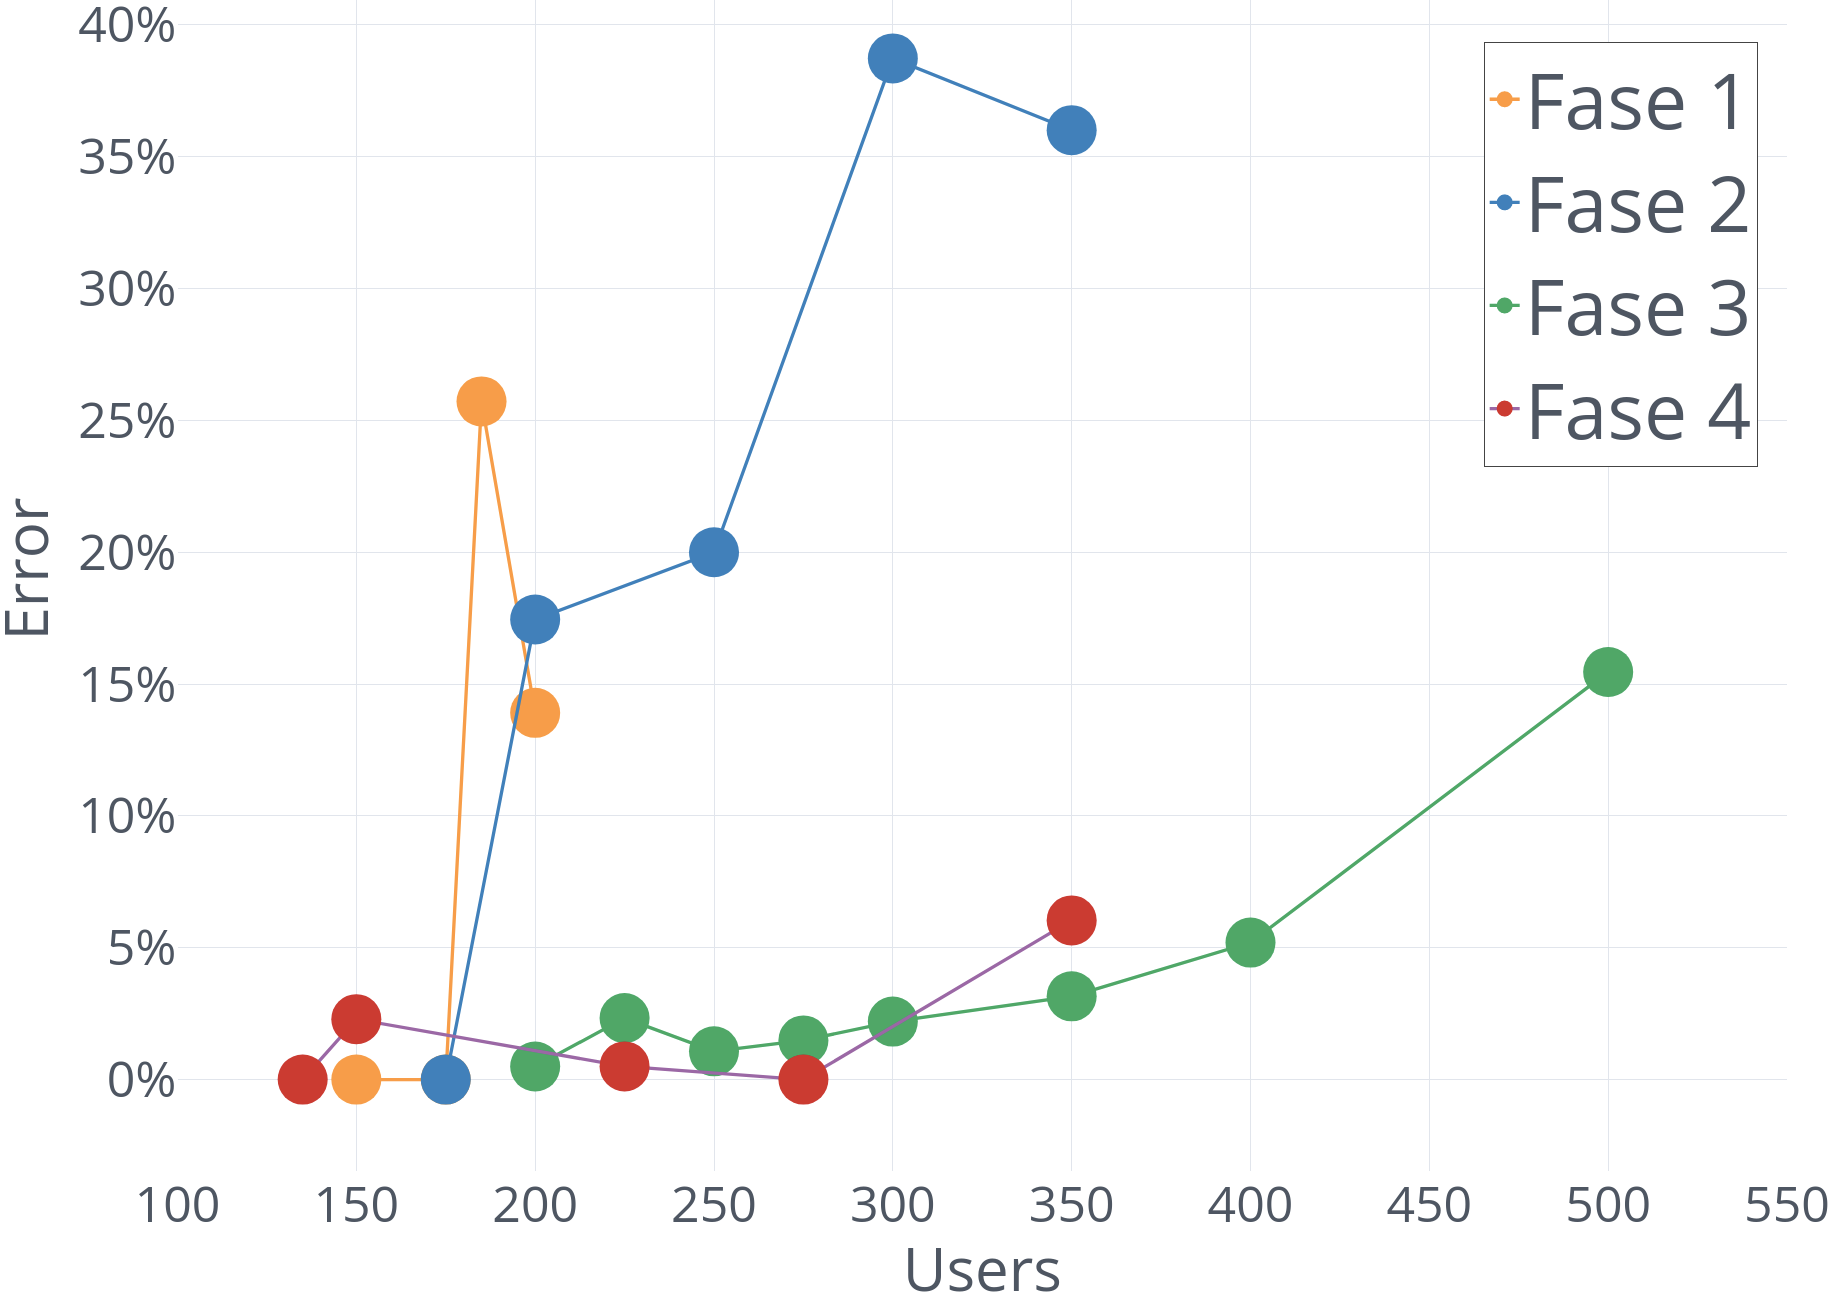
\includegraphics[width=1\linewidth]{Chapters/img/testing/1Pod.png} 
    \caption{One Pod} 
    \label{fig:1pod}
    \vspace{1ex}
  \end{minipage}%%
  \begin{minipage}[b]{0.5\linewidth}
    \centering
    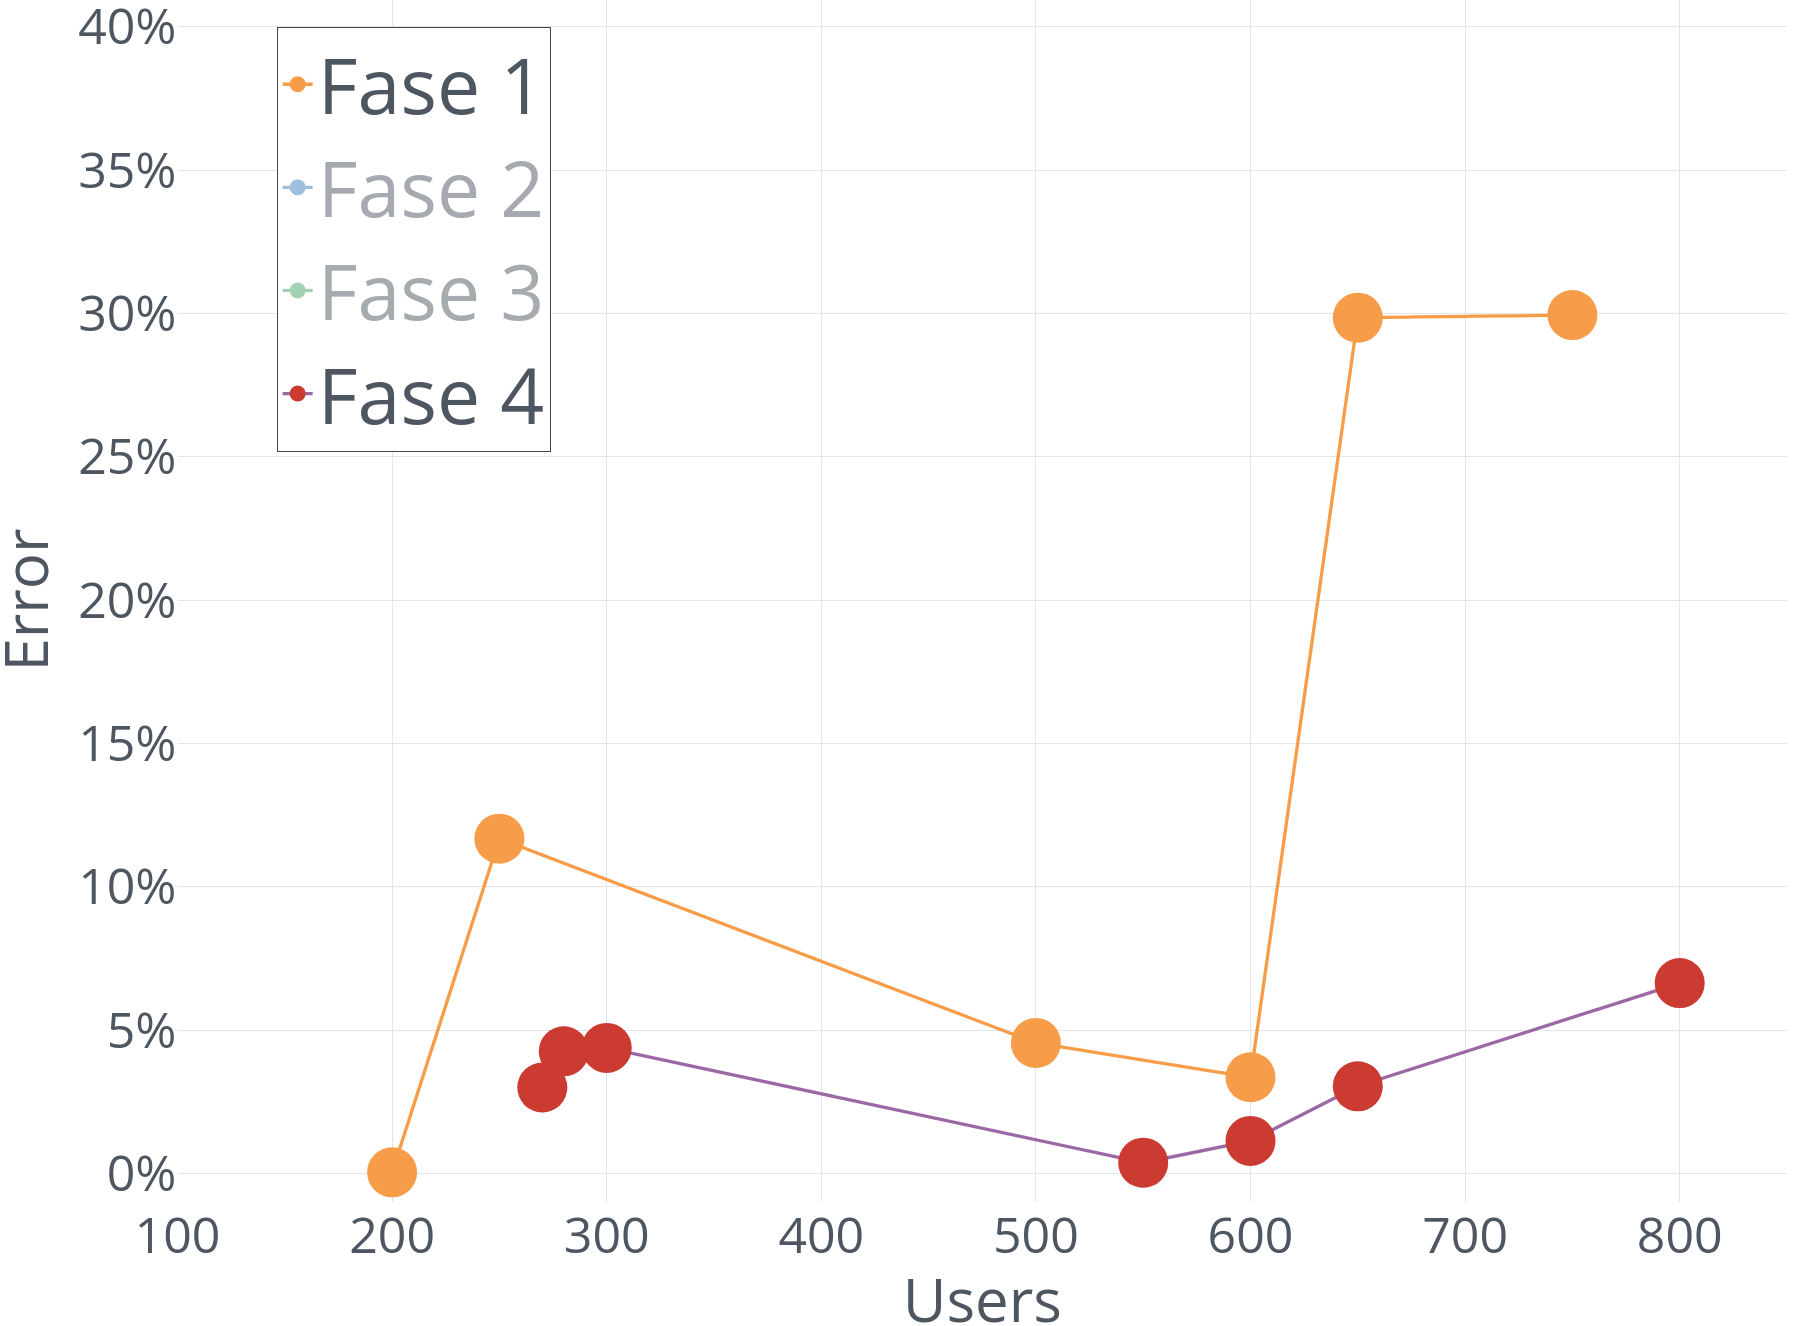
\includegraphics[width=1\linewidth]{Chapters/img/testing/2Pod.png} 
    \caption{Two Pods} 
    \label{fig:2pods}
    \vspace{1ex}
  \end{minipage} 
\end{figure}

The \textbf{first testing phase}, represented in orange, allowed us to understand that abundant resources would not suffice as the results were subpar, with an error rate above 10\% for 200 concurrent users. In this test, the pods were setup with 800 \acrfull{m} of CPU and 800 \acrfull{mib} of RAM.

During this phase, it was possible to observe that only 50\% of the pod memory was being utilized, so during \textbf{phase two (blue)}, we increase \acrshort{jvm} memory options to access 75\% of the available RAM. The change ended up with not affecting the error rate, proving that just adding more resources would not solve the problem, however it allowed for resource optimization, saving scarce resources.

From the previous tests, we came to the conclusion that the ideal memory values would be 400MB for the \acrshort{jvm}, from the 500\acrshort{mib} provided to the pod. With the ideal memory values found, we could now try to optimize the CPU which was given access to 1 entire core per pod, decreasing the error rate to below 5\% for 200 and 350 users, as can be observed in Fig. \ref{fig:1pod} during \textbf{phase three (green)}. This change also had an effect in the boot speed, which decreased from 50 seconds to an average of 30 seconds, and led us to test how different CPU resources affect boot speed.

All microservices were written in \textbf{Java} and include the \textbf{Spring} framework, which on average (observed from our services in idle), require about 120-200 \acrfull{mib} while online, with the most demanding ones using 500 \acrshort{mib} at peak load. The most problematic aspect when dealing with Spring is the boot time, strongly affected by the amount of CPU allocated to it. By testing, we were able to gather the following results, displayed on table \ref{tbl:cpuBoot}.

\begin{table}[!h]
    \centering
    \begin{tabular}{c|c}
    CPU (cores) & Boot (sec)  \\ \hline
    500m        & $\sim$120 \\
    800m        & $\sim$70  \\
    1000m       & $\sim$30 
    \end{tabular}
    
    \caption{Relation between processing power (CPU) and boot time}
    \label{tbl:cpuBoot}
\end{table}

As \acrshort{k8s} does not hoard the resources if not in use, as long as not explicitly told to do so, we decided to allow each pod access to one entire core. This way, we have resources for a fast boot, while also not wasting resources when they are idle as CPU usage is reduced to about 10 \acrshort{m}.

Still during phase three we have noticed that after booting up, the pods were using 300\acrshort{mib} of RAM that would slowly increase until running out of memory and crashing. To try and fix it, we experimented with a different garbage collector Garbage First Garbage Collector (G1GC), which actually started releasing memory when it was no longer necessary, increasing the pod uptime and error rate, observed in \textbf{phase four (red)}.

This phase provided the best results with \textbf{275 users with a 0\% error rate}, upon completing this stress test and finding the limit of our pod, we could now proceed with the next round of tests, where we try out the optimal configurations found for the pods. Which resulted in phase four (red) in Fig. \ref{fig:2pods}, which was an improvement over its phase one results allowing up to \textbf{600 users with a sub 2\% error rate}.

With the ideal pod configuration found and the pod user limits discovered, we can now focus on the scalability testing to understand how the system reacts to changes in the number of simultaneous users. The following metrics were chosen to test as scaling parameters:

\begin{enumerate}
    \item \textbf{http\_server\_requests\_seconds\_count} --- represents the number of requests received at a certain endpoint at a given time;
    \item \textbf{CPU usage} --- represents the CPU processing power being used at a given time;
    \item \textbf{http\_server\_requests\_seconds\_max} --- represents the maximum request duration during in a rolling window, as such the purpose is to measure the worst outlier, following the work of F. Rossi et al~\cite{rossi2020hierarchical}.
\end{enumerate}

And, as a way to optimize our solution, the following rules have been defined: 
It was also necessary to define some of the rules the system must follow, to ensure no resources were wasted and they fit within the findings discovered earlier in single pods testing.

\begin{itemize}
    \item Scaling up to two pods, only when the load is higher or similar to the ceiling found during our one pod test (e.g., should not scale with less than 200 users);
    \item The pods should be given a grace period to scale up, where they can handle the full load while the second pod is loading up without losing any requests;
    \item Handle almost the same load as the experiment that ran with two deployed pods.
\end{itemize}

\begin{figure}[h]
    \centering
    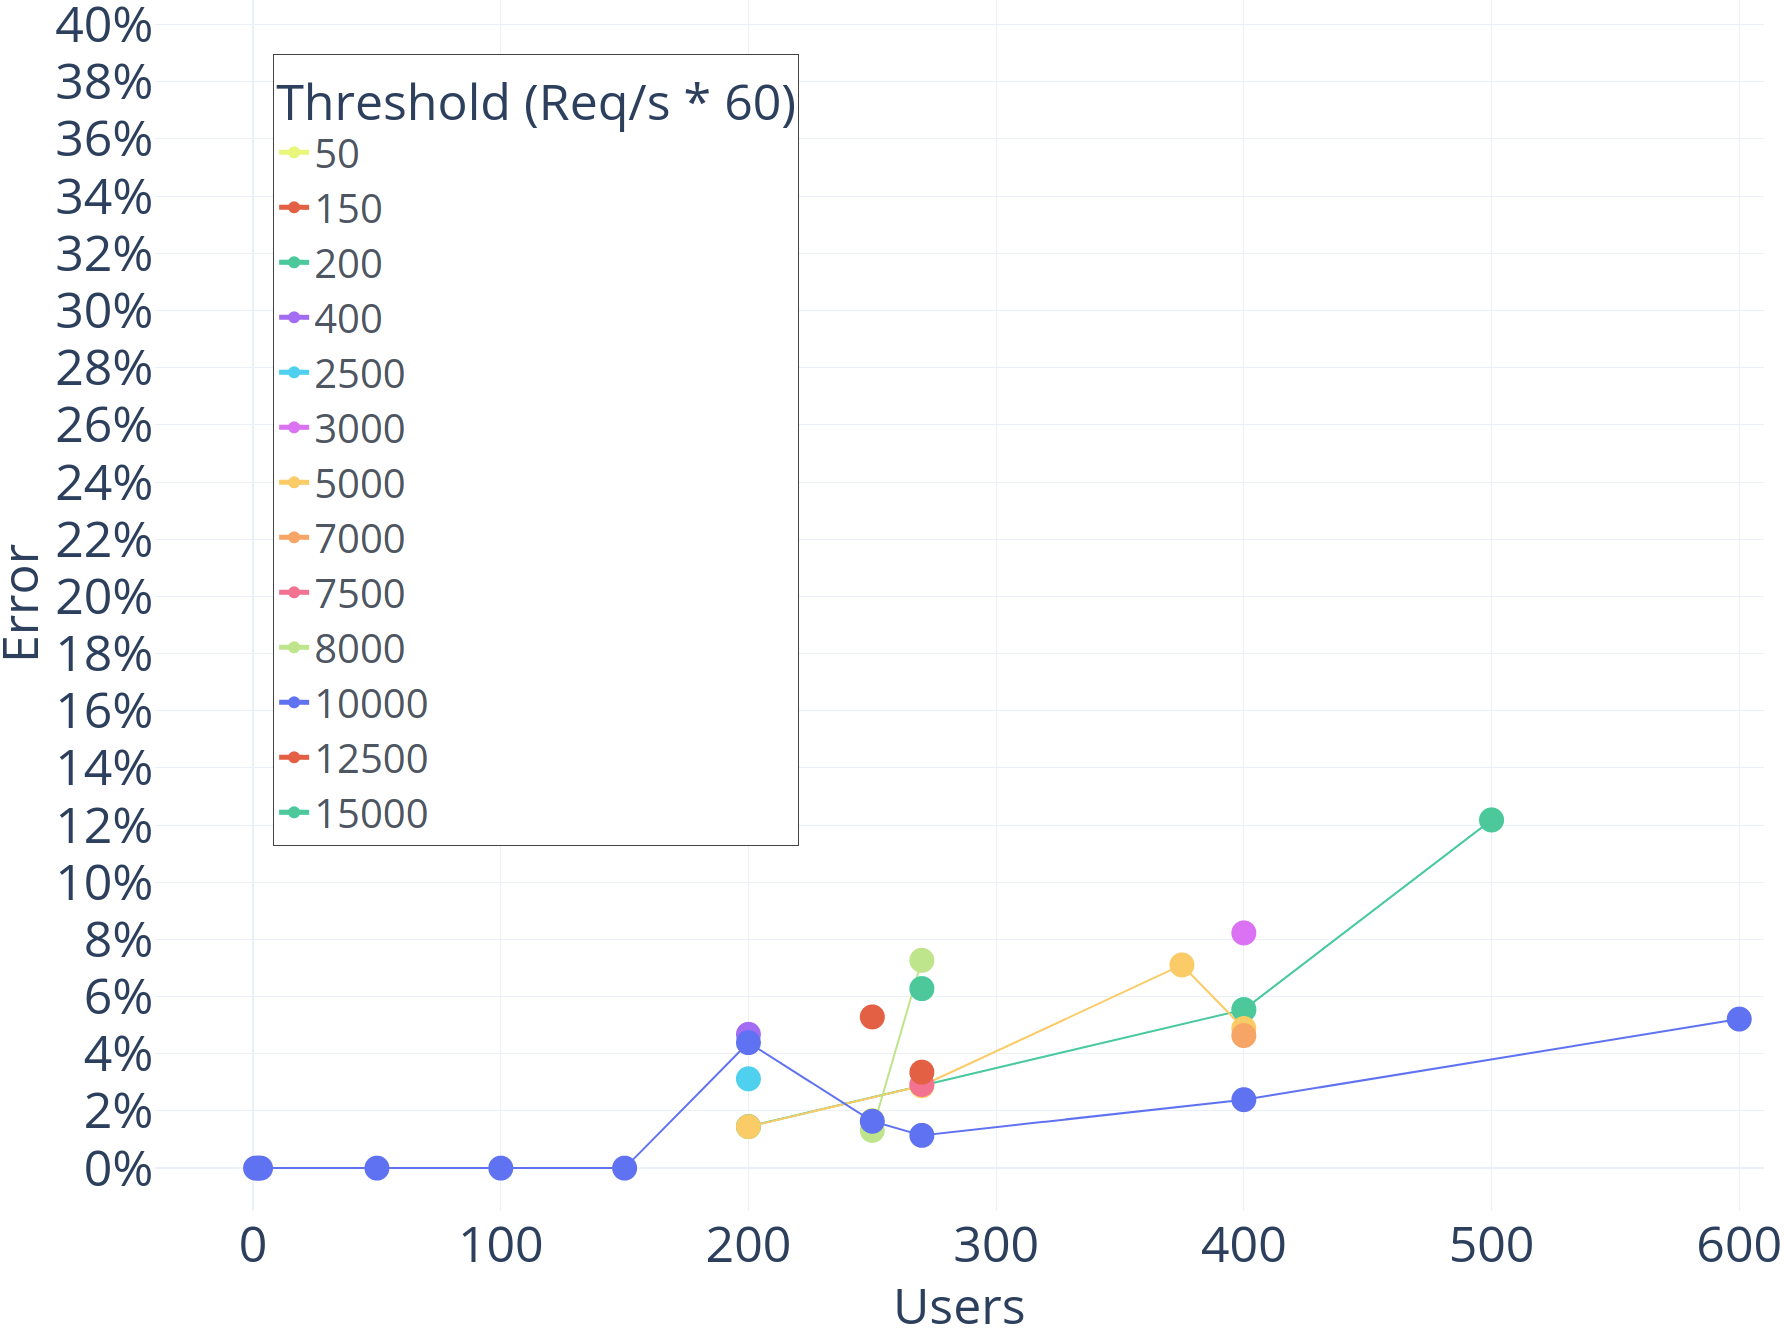
\includegraphics[width=0.5\textwidth]{Chapters/img/testing/HPA_HttpCountIncreaseLeft.png}
    \caption{Increase of HTTP Requests}
    \label{fig:metric_increase}
\end{figure}

As stated previously, the first metric tests a scenario where the system would scale based on the number of requests received, which can be seen in Fig. \ref{fig:metric_increase}. Over this metric, the Prometheus function \textbf{Increase} has been applied to a 1 minute window, which calculates the per-second average rate of increase of the time series in that interval and multiplies its value by the defined interval in seconds (60). In the mentioned figure, it is possible to observe that tests with more than 300 concurrent users had an error rate above 7.5\%, independent of the chosen threshold. In addition, we noticed that the pods were scaling even when below 200 concurrent users, breaking the first rule.

Despite the metric not meeting the defined requirements, it helped us realize that we were losing requests during the scaling period due to \acrshort{k8s} routing requests to newly instantiated pods. This happened because the pod was declared ready when \acrshort{jvm} launched, but not before Spring finished up booting up. To fix it, we had to swap the default implementations of the Readiness and Liveness probes, to the ones exposed through the Micrometer library. This way, pods are only declared ready and alive, when Spring is ready to process requests.

%Over the first metric, Fig.~\ref{fig:metric_increase}, the Prometheus function \textbf{Increase} has been applied with a 1 minute window, which calculates the per-second average rate of increase of the time series in that interval and multiplies its values by the defined interval in seconds (60). As seen in our figure, most of the tests with more than 300 users had an error rate above 7.5\%, independent of the chosen threshold. We also noticed that even when using values below 200 (way below our 1 pod threshold found previously), the pods would scale anyway, which violates one of our requirements. 

%Even though the metric didn't meet the defined requirements, it allowed us to realize that we were losing requests during the scaling period because Kubernetes was routing requests to the newly instantiated pod, as it was declared ready when JVM launched but before Spring finished booting up. We then implemented new readiness and liveness probes, based on the micrometer metrics, which allowed us to declare the pod as ready and alive only when Spring actually launches and is ready to process requests.

\begin{figure}[h]
    \centering
    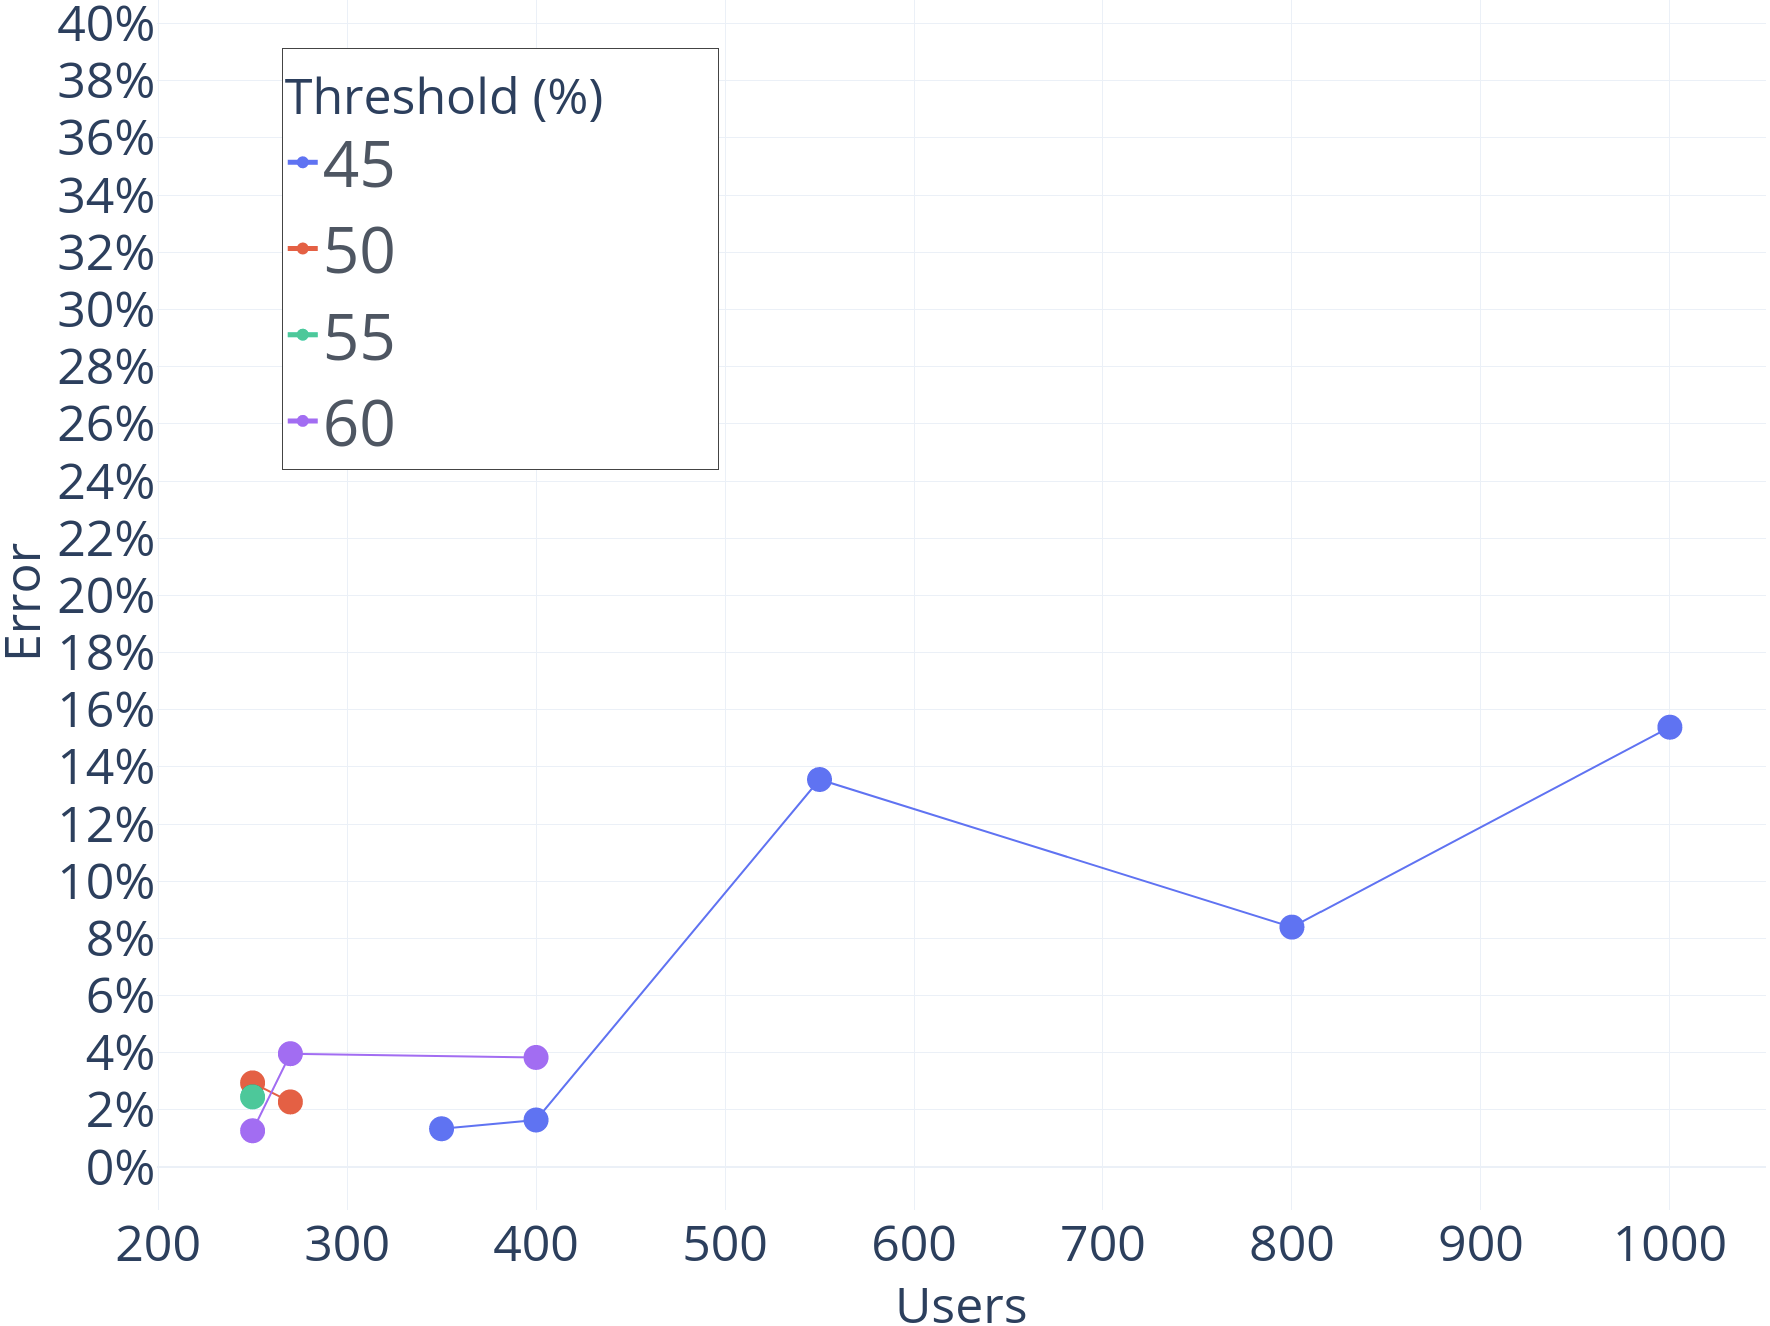
\includegraphics[width=0.5\textwidth]{Chapters/img/testing/HPA_CpuUsageLeft.png}
    \caption{Percentage of CPU usage}
    \label{fig:metric_cpu}
\end{figure}

For the second test, Fig. \ref{fig:metric_cpu}, the scaling was based on \textbf{CPU Usage}. We noticed that for the most part, the pod CPU usage was always at max load while receiving requests, which caused the cluster to immediately scale, independently of the number of concurrent users, explaining the poor results displayed.

%The second metric, \textbf{CPU usage} Fig.~\ref{fig:metric_cpu}, displayed poor results since CPU usage was for the most part, always at max load, which caused our cluster to immediately scale even though it was unnecessary. 

\begin{figure}[h]
    \centering
    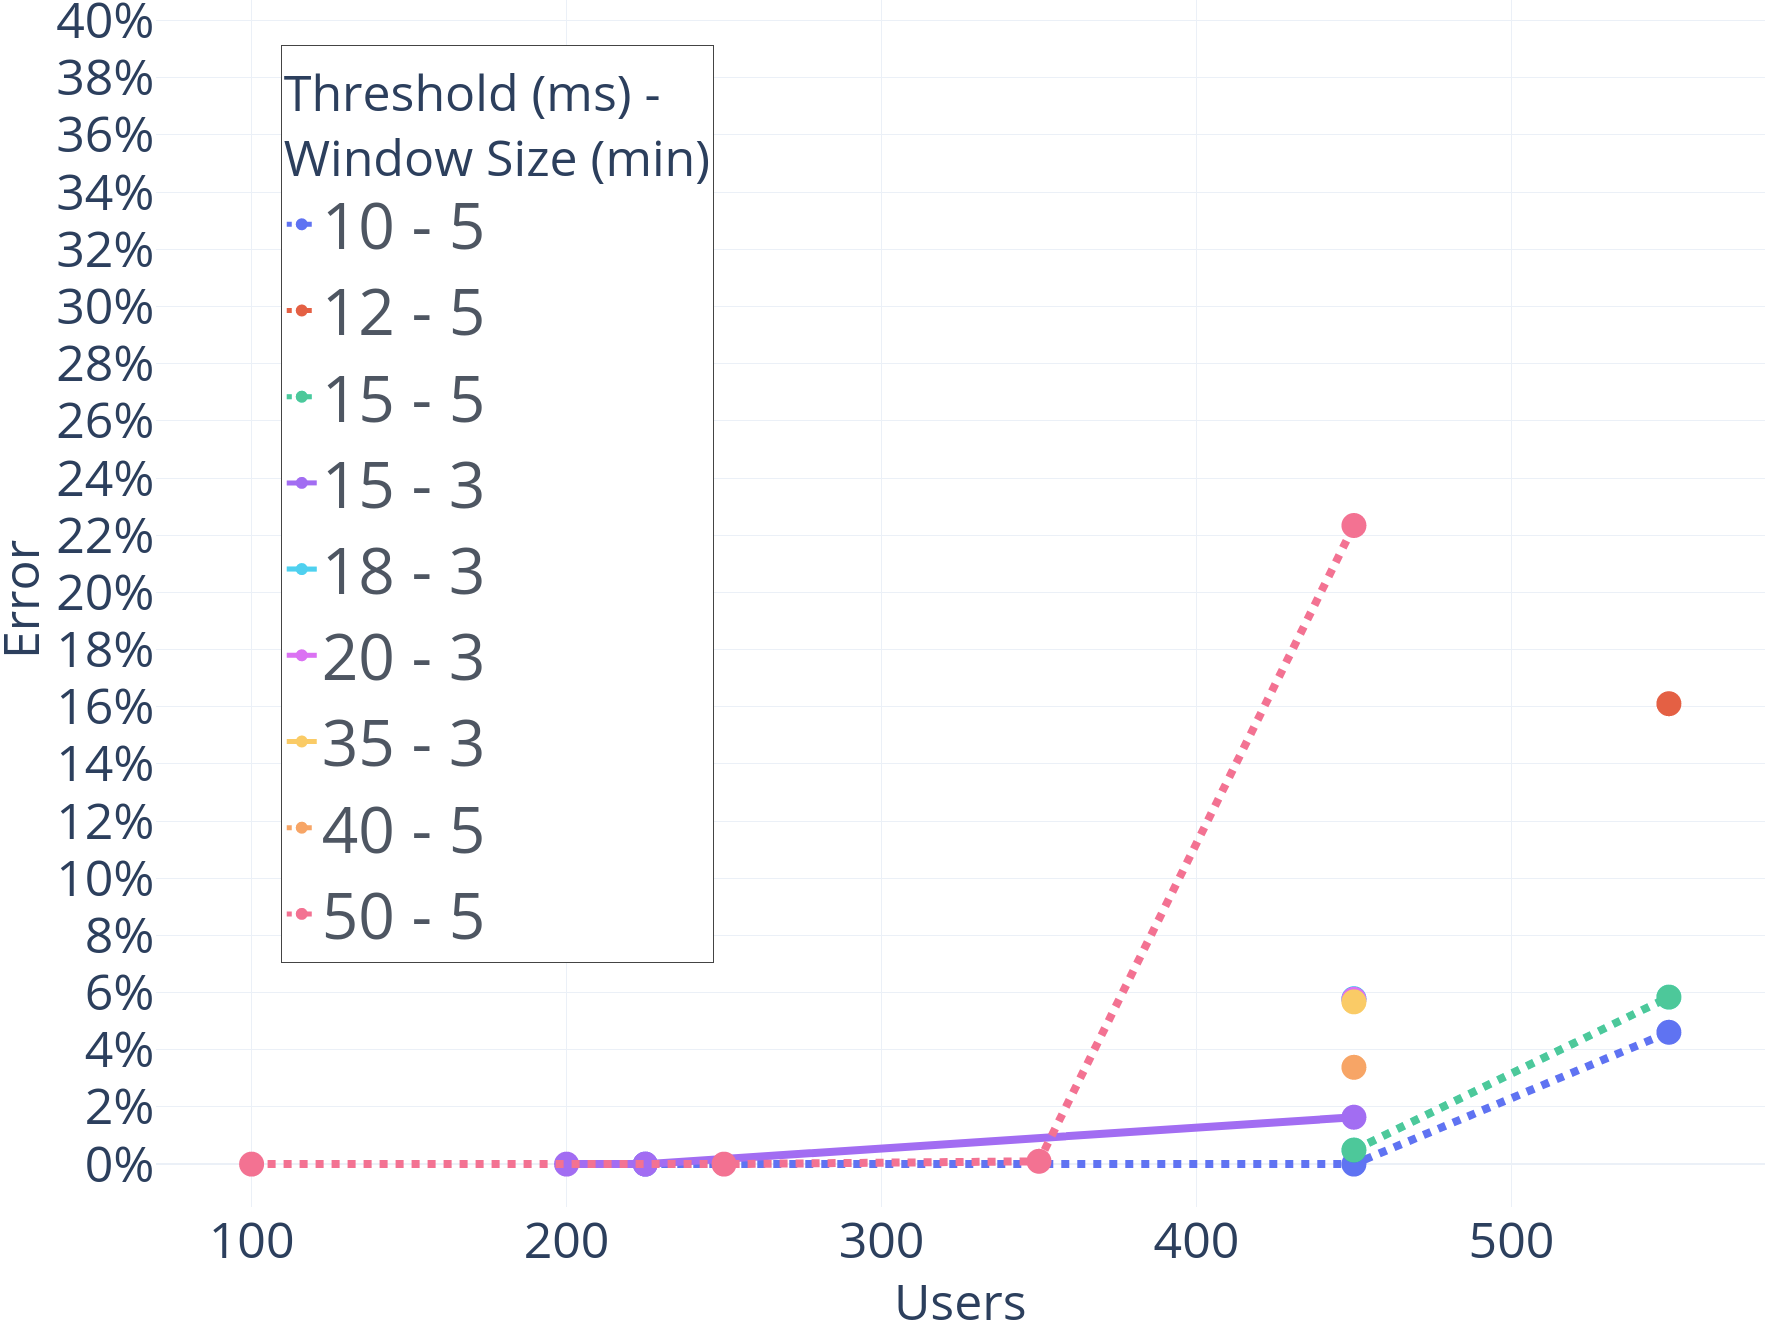
\includegraphics[width=0.5\textwidth]{Chapters/img/testing/HPA_HttpMaxRateLeft.png}
    \caption{Rate of MaxResponseTime}
    \label{fig:metric_max}
\end{figure}

For the final test, we experimented with \textbf{http\_server\_requests\_seconds\_max} extracted from the Micrometer library. On top of this data, we applied a Prometheus rate which calculates the per-second average rate of increase within a certain interval. We performed tests with 3 and 5 minute window intervals as observer in Fig. \ref{fig:metric_max}, with normal and dotted lines, respectively. 

In the same figure it is possible to observe that the 5 minute window produces good results, but, similarly to the results of the first metric, it would scale even when below the 200 users threshold, breaking our defined rule. Additionally, given the window size of the rate function, adjusting the threshold would not help as the test would be over by the time it would stabilize.

As such, we tried reducing the window to 3 minutes and increase the threshold to 50 to try and avoid unnecessary scaling, which backfired by never scaling, even when above 400 concurrent users. Trying different thresholds (40, 35, 20 and 18) while maintaining the same number of users (450) produced results by progressively decreasing the error rate to below 5\%, but still above the desired value of 2\%.

Based on these results, it led us to the 15ms threshold, where it managed to hold a \textbf{sub 2\% error rate with 450 users} and sustain, at least, 200 concurrent users without triggering the scaling process. As a final experiment, to confirm the results, the test duration was increased to 10 minutes and it managed to maintain the same error rate.






%\subsubsection{Scalability}
%\label{ss:scalability}

%\subsubsection{Load}
%\label{ss:load}

%\subsection{Usability}
%\label{s:usability}

%\todo[inline]{Fazer testes de usabilidade da aplicação com 15 a 30 pessoas}
%\todo[inline]{Avaliar eficácia do sistema de recomendaçoes}

% Fazer testes de usabilidade da aplicação com 15 a 30 pessoas
% Avaliar eficácia do sistema de recomendaçõe